\subsection{Glasfaser (H.G.)}
\label{Glasfaser}
Glasfasern gelten als älteste synthetische Faserart und wurden schon vor 3500 Jahren verwendet. Heutzutage werden Glasfasern überwiegend aus SiO2 und Metalloxiden hergestellt. Die Bestandteile werden bei ca. 1400°C aufgeschmolzen und durch kleine Düsen im Boden des Kessels als dünne Fäden ausgelassen. Die Fäden werden aufgewickelt und zu größeren Fasern versponnen\cite{item3}.
Die hohe Festigkeit der Glasfaser beruht auf den kovalenten Bindungen von Silizium- und Sauerstoff-Atomen. Zugesetzte Metalloxide verhindern eine Ausbildung eines geordneten Gefüges und erhöhen somit zusätzlich die Festigkeit. Die Fasern können in Längsrichtung sehr hohe Kräfte aufnehmen, jedoch nicht in Querrichtung. Deshalb werden sie in eine Matrix integriert, die die Querkräfte aufnimmt und die Faser vor dem Knicken schützt. Glasfasern lassen sich auch um enge Radien sehr gut drapieren und sind durch ihre einfache Herstellungsweise im Vergleich zu anderen Faserarten sehr preiswert \cite{item4}.
Durch die zuvor erläuterten Eigenschaften sind Glasfasern sehr gut für dieses Projekt geeignet, für einen größeren Flügel wäre jedoch der Elastizitätsmodul zu gering und es müsste auf andere Fasern, wie zum Beispiel Kohlefasern, zurückgegriffen werden. 
Für die Konstruktion des Flügels stehen die Glasfasern Interglas 90070 (bidirektional) und Interglas 92145 (idealisiert unidirektional) des Herstellers Interglas Technologies zur Verfügung. 

\subsection{Matrix (H.G.)}
Unter der Matrix versteht man den Fasern umgebenden Teil des Faserverbundstoffs. Dabei werden im Bereich des Faser-Kunststoff-Verbunds Polymere, wie z.B. Epoxidharz, verwendet. Die Matrix ist meist der schwache Teil des FKV und hat die Aufgabe, die Fasern gegen Knicken bei Druckbelastung zu schützen und eine gleichmäßige Krafteinleitung in die Fasern zu ermöglichen. Zusätzlich hält sie die Fasern in Position und verhindert Reibung zwischen den einzelnen Fasern \cite{item3}.\\
Für den Flügel wird der Epoxy-Kunststoff L 385 des Herstellers \textit{MGScheufler} zusammen mit dem Härter H 386 im Mischverhältnis 100/40 verwendet.
\subsection{Netztheorie (H.G.)}
Bevor die klassische Laminattheorie entwickelt wurde, verwendete man die sogenannte Netztheorie. 
Bei der Netztheorie wird das Mittragen der Matrix vernachlässigt. Dadurch lassen sich die Schichtkräfte mit Hilfe eines Kräftegleichgewichts bestimmen. 
Durch diese Vereinfachungen kann der Konstrukteur schnell feststellen, ob die Fasern alleine der Belastung standhalten können. Wenn dies nicht der Fall ist werden die Kräfte größtenteils über die Matrix übertragen und das Laminat wird als \textit{ungesund} bezeichnet. Durch die Annahme, dass die Matrix nicht tragend ist, wird das Laminat jedoch unterschätzt und weist deutlich höhere Festigkeiten auf, als in der Netztheorie angenommen. Damit wird in jedem Fall eine Sicherheit mit eingerechnet.\\
Für die Verwendung der Netztheorie sollte das Gelege zunächst in ein Hauptachsenkoordinatensystem überführt werden, damit die Schubspannungen verschwinden. Die Kraftflüsse werden damit zu $\hat{n}_{I}$ und $\hat{n}_{II}$. Nun lässt sich der Winkel $\beta $ zwischen den Fasern und den Achsen des Hauptachsenkoordinatensystems bestimmen. Mit diesem und der Annahme, dass nur die Spannungen $\sigma_{\|}$ auftreten, können nun die Schnittkräfte in den Fasern bestimmt werden:
\begin{equation}
\hat{n}_{I}=\sum n_{\|k}\cdot cos^2\beta_{k}
\end{equation}
\begin{equation}
\hat{n}_{II}=\sum n_{\|k}\cdot sin^2\beta_{k}
\end{equation}
\begin{equation}
0=\frac{1}{2}\sum n_{\|k}\cdot sin2\beta_{k}.
\end{equation}
Da der gesamte Kraftfluss als Summe der Kraftflüsse in den einzelnen Fasern angenommen werden kann, lässt sich dadurch der Kraftfluss in den einzelnen Faserschichten und somit die benötigte Dicke der Schichten, bzw. die Anzahl der Lagen bestimmen\cite{item3}.

\noindent In der folgenden Berechnung wird die Netztheorie jedoch nicht verwendet, da die Auslegung vorerst mit der VDI 2013 erfolgt und anhand der Klassischen Laminattheorie.
\subsection{Klassische Laminattheorie (H.G.)}\label{CLT}
Das Prinzip der klassischen Laminattheorie ist die Beschreibung des Elastizitätsgesetzes eines MSV durch die Elastizitätsgesetze der einzelnen Schichten. Dies lässt sich durch die Annahme eines ideal elastischen und fehlerfrei verklebten Mehrschichtverbund (MSV), wovon ein infinitesimales Scheibenelement betrachtet wird, realisieren. Zusätzlich gilt die Annahme, dass ein ebener Spannungszustand vorliegt, die Schnittspannungen über die Dicke konstant sind und keine Verwölbungen auftreten.\\
\noindent
Der Kraftfluss $\hat{n}$ im ganzen Laminat lässt sich durch die Summe der Kraftflüsse in den einzelnen Schichten zusammensetzen.
\begin{equation}
\label{Kraftfluss}
\hat{n}_{x}=\hat{\sigma}_{x}\cdot t=\sum n_{xk}=\sum\sigma_{xk}\cdot t_{k}
\end{equation}

\begin{equation}
\hat{n}_{y}=\hat{\sigma}_{y}\cdot t=\sum n_{yk}=\sum\sigma_{yk}\cdot t_{k}
\end{equation}

\begin{equation}
\hat{n}_{xy}=\hat{\tau}_{xy}\cdot t=\sum n_{xyk}=\sum\sigma_{xyk}\cdot t_{k}
\end{equation}
Nun lässt sich das Elastizitätsgesetz für den MSV aufstellen:
\begin{equation}
\label{Aep}
\lbrace \hat{n}\rbrace= [A]\cdot \lbrace\hat{\varepsilon}\rbrace .
\end{equation}
$[A]$ ist hierbei die Steifigkeitsmatrix des MSV. Mit Hilfe der Kraftfluss- Spannungsbeziehung aus Gleichung \ref{Kraftfluss}, lässt sich dann auf die Spannung schließen.
\begin{gather}
\begin{Bmatrix}
\hat{\sigma}_{x}\\
\hat{\sigma}_{y}\\
\hat{\tau}_{xy}\\
\end{Bmatrix}
=
\frac{1}{t}
\begin{bmatrix}
A_{11}&A_{12}&A_{16}\\
A_{12}&A_{22}&A_{26}\\
A_{16}&A_{26}&A_{66}
\end{bmatrix}
\cdot
\begin{Bmatrix}
\hat{\varepsilon}_{x}\\
\hat{\varepsilon}_{y}\\
\hat{\gamma}_{xy}\\
\end{Bmatrix}
\end{gather}
\noindent
Die Verzerrung des MSV und somit auch die Verzerrung der Einzelschichten, lässt sich nun durch die Umstellung von Gleichung \ref{Aep} bestimmen.
\begin{equation}
\label{SpannungDehnung}
\lbrace\hat{\varepsilon}\rbrace = [A]^{-1}\cdot\lbrace \hat{n}\rbrace
\end{equation}
\noindent
Um die Matrix A zu bestimmen werden die Steifigkeitsmatritzen der Einzelschichten $[Q]$ benötigt. Diese lassen sich mit Hilfe der E-Moduln, Querkontraktionszahlen definieren.
\begin{equation}
[Q]
=
\begin{bmatrix}
\frac{E_{\|}}{1-\nu_{\bot\|}\cdot \nu_{\|}\bot}&\frac{\nu_{\bot\|}\cdot E_{\bot}}{1-\nu_{\bot\|}\cdot \nu_{\|}\bot}&0\\
\frac{\nu_{\|\bot}\cdot E_{\|}}{1-\nu_{\bot\|}\cdot \nu_{\|}\bot}&\frac{E_{\bot}}{1-\nu_{\bot\|}\cdot \nu_{\|}\bot}&0\\
0&0&G_{\bot\|}
\end{bmatrix}
\end{equation}
\noindent
Da manche Faserschichten um einen Winkel $\alpha$ gedreht sein können, muss für diese Schichten die Steifigkeitsmatrix mit Hilfe der Transformationsmatrix $[T]$  nach der Transformationsregel aus Gleichung \ref{trafo} transforniert werden.
\begin{equation}
	\underline{\underline{T}}=
	\begin{bmatrix}
		\cos^{2}\alpha&\sin^{2}\alpha&-\sin 2\alpha\\
		\sin^{2}\alpha&\cos^{2}\alpha&\sin 2\alpha\\
		0,5\cdot \sin2\alpha&-0,5\cdot\sin2\alpha&\cos 2\alpha
	\end{bmatrix}
\end{equation}\\
\begin{equation}
\label{trafo}
	\overline{\underline{\underline{Q}}}=\underline{\underline{T}}\cdot \underline{\underline{Q}} \cdot \underline{\underline{T}}^{T}  
\end{equation}\\
\noindent
Nun lässt sich die Scheibensteifigkeits-Matrix [A] aus den Steifigkeitsmatritzen der einzelnen Schichten zusammensetzen (siehe Glg.\ref{AQ}).
\begin{equation}
\label{AQ}
	A_{ij}= \sum_{k=1}^{2} \overline{Q}_{ij,k}\cdot t_{k}
\end{equation}
\noindent
Um ein passende Anzahl an Faserschichten zu bekommen kann das Ergebnis nun iterativ angepasst werden.\cite{item3}
\subsubsection{Ingenieurskonstanten des MSV}
Für den einachsigen Spannungszustand lassen sich die Moduln und Querkontraktionszahlen für den MSV ableiten.
Diese lassen sich experimentell über z.B. einen Zugversuch oder rechnerisch aus dem Elastizitätsgesetz des MSV bestimmen.
\begin{equation}
\hat{E}_{x}=\frac{1}{A_{11}^{-1}\cdot t}
;
\hat{E}_{y}=\frac{1}{A_{22}^{-1}\cdot t}
;
\hat{G}_{xy}=\frac{1}{A_{66}^{-1}\cdot t}
;
\hat{\nu}_{xy}=-\frac{A_{12}^{-1}}{A_{22}^{-1}}
;
\hat{\nu}_{yx}=-\frac{A_{12}^{-1}}{A_{11}^{-1}}
\end{equation}
\noindent
Die Spannungen lassen sich jetzt durch Gleichung \ref{SpannungDehnung} errechnen.\\
\noindent
Bei den Elastizitätsmoduln ist darauf zu achten, dass es sich um Moduln ohne Querkontraktionsbehinderung handelt \cite{item3}.
\subsubsection{Plattenelement}
Um ein Plattenelement zu Berechnen werden zusätzliche Beziehungen benötigt, da nun ein zweiachsiger Spannungszustand vorliegt. Zu Gleichung \ref{AQ} kommen nun noch 2 weitere Gleichungen (siehe Glg.\ref{BQ}/\ref{DQ}) hinzu.
\begin{equation}
\label{BQ}
	B_{ij}= \cdot \sum_{k=1}^{2} \overline{Q}_{ij,k}\cdot t_{k}\cdot \left(z_{k}-\frac{t_{k}}{2}\right)
\end{equation}
\begin{equation}
\label{DQ} 
	D_{ij}=\sum_{k=1}^{2} \overline{Q}_{ij,k}\cdot \left(\frac{t_{k}^{3}}{12}+t_{k}\left(z_{k}-\frac{t_{k}}{2}\right)^{2}\right)
\end{equation}
\noindent
Nun lässt sich die Scheiben-Platten-Beziehung als Gleichung \ref{S-P} schreiben.\cite{item3}
\begin{equation}
\label{S-P}
	\begin{pmatrix}
		\hat{\underline{n}}\\
		\hat{\underline{m}}
	\end{pmatrix}
	= \begin{bmatrix}
		\underline{\underline{A}}&\underline{\underline{B}}\\
		\underline{\underline{B}}&\underline{\underline{D}}
	\end{bmatrix}
	\cdot \begin{pmatrix}
		\underline{\epsilon}\\
		\underline{\kappa}
	\end{pmatrix}
\end{equation}\\



\subsection{Mischungsregel (H.G.)}
Um die Materialkonstanten des FKV zu ermitteln kann die Mischungsregel verwendet werden. Darin werden die Materialkonstanten der Fasern und der Matrix im Verhältnis zu ihrem Massenanteil zu einer FKV-Materialkonstante zusammengestellt.\\
\noindent
Die Dichte des FKV lässt sich aus der Dichte der einzelnen Komponenten errechnen (siehe Glg. \ref{dichte}).
\begin{equation}
\label{dichte}
	\rho=\rho_{F}\cdot\varphi +\rho_{M}\cdot (1-\varphi)
\end{equation}
\noindent
Der E-Modul parallel (siehe Glg. \ref{Eparallel}) und orthogonal (siehe Glg. \ref{Eorthogonal}) kann mit den E-Modulen von Faser und Matrix, sowie dem Faservolumenanteil $\varphi$ errechnet werden. Zu betonen ist hierbei, dass auf eine Querkontraktionsbehinderung der Matrix durch die Fasern nicht eingegangen wird. In diesem Fall wären die resultierenden Steifigkeiten größer. Um sicher konservativ rechnen zu können, wird demnach die vereinfachte Rechnung benutzt. Aus selbigem Grund wird daher auch auf höhere Mischungsregeln, wie z.B. nach Puck, verzichtet. 
\begin{equation}
\label{Eparallel}
E_{\|}=E_{f\|}\cdot \varphi+E_{m}\cdot (1-\varphi)
\end{equation}

\begin{equation}
\label{Eorthogonal}
E_{\bot}=\frac{E_{m}}{(1-\varphi)\cdot\frac{E_{m}}{E_{f\bot}}\cdot\varphi}
\end{equation}
\noindent
Der Schubmodul in Faser-Quer-Längs-Richtung kann ebenfalls durch die Schubmodule der Fasern und der Matrix ermittelt werden.
\begin{equation}
G_{\bot\|}=G_{m}\frac{1}{(1-\varphi)+\frac{G_{m}}{G_{f\bot\|}}\cdot\varphi}
\end{equation}
Außerdem lassen sich die Querkontraktionszahlen berechnen.
\begin{equation}
\nu_{\bot\|}=\varphi\cdot \nu_{f\bot\|}+(1-\varphi)\cdot \nu_{m}
\end{equation}
Aus diesen Werten lassen sich alle weiteren durch die Beziehungen zwischen den Materialkonstanten berechnen.\cite{item3}

\subsection{Versagenskriterium nach Puck (O.S.)}
Da für einen anisotropen FKV nicht das Versagen mittels einer allgemeinen resultierenden Spannung für jeden Lastfall ermittelt werden kann, müssen Versagenskriterien für die speziellen Beanspruchungsmodi definiert werden. Für die in dieser Projektarbeit durchgeführten Auslegungen wurden die Festigkeitskriterien von Puck verwendet. Hierbei werden die einzelnen UD-Schichten des Laminats getrennt betrachtet. Auch wenn diese Betrachtungen physikalisch begründet sind (vgl. \cite{EdL}), hat dies zur Folge, dass Effekte wie Delamination nicht berücksichtigt werden.
\subsubsection{Definitionen}
Zunächst sind einige Begriffe zu definieren. An einer UD-Schicht können zwei verschiedene Normalspannungen wirken, die sich, je nachdem, ob es sich um Druck- oder Zugbelastung handelt, unterschiedlich auf das Versagen auswirken: die Längsbeanspruchung $\sigma_{\parallel}$ parallel und die Querbeanspruchung $\sigma_{\perp}$ orthogonal zur Faserrichtung. Auch bei der Schubspannung muss zwischen der Quer-/Quer-Schubbeanspruchung $\tau_{\perp\perp}$ und der Längs-/Quer-Schubbeanspruchung $\tau_{\parallel\perp}$ unterschieden werden. Wegen des durch die Fasern bedingten stark anisotropen Aufbaus muss zwischen zwei grundlegenden Versagensarten unterschieden werden: dem Faserbruch (Fb) und dem Zwischenfaserbruch (Zfb). Der Begriff Bruch ist hier bewusst als Schadensbezeichnung gewählt, da bei beiden Fällen kein plastisches Verhalten auftritt und es sich um einen Sprödbruch ohne nennenswertes Fließen handelt.
Für das Versagenskriterium wird die genaue Definition der Anstrengung $f_E$ gesucht. Diese ist abhängig vom Spannungszustand und immer so definiert, dass bei $f_E=1$ das Versagen eintritt, sie also bei Belastungen, die das Material, aushält Werte kleiner als $1$ und bei überkritischen Lasten größer $1$ annimmt.

\noindent Beim Zfb stimmt die Bruchebene nicht unbedingt mit der Wirkebene, der Ebene mit der höchsten Beanspruchung, überein. Auf anderen Ebenen können andere Festigkeiten herrschen, die früher überschritten werden. Generell gilt für sie, dass die Bruchebene immer parallel zu den Fasern sein muss. Puck führt analog zur Festigkeit den Bruchwiderstand der Wirkebene $R^A$, der als "derjenige Widerstand [definiert ist], den eine Schnittebene ihrem Bruch infolge einer einzelnen in ihr wirkenden Beanspruchung (bei Zfb: $\sigma_\perp^+$ oder $\tau_{\perp\perp}$ oder $\tau_{\parallel\perp}$) entgegensetzt"\cite{item3}.
\subsubsection{Zwischenfaserbruch ohne Längsspannung}
Ignoriert man die Längsspannung $\sigma_1$, da diese erst bei sehr hohen Werten Einfluss auf einen Zfb hat, ergibt sich ein Spannungszustand aus den beiden übrigen Normalspannungen $\sigma_2$ und $\sigma_3$ orthogonal zu den Fasern und den Schubspannungen $\tau_{12}$, $\tau_{23}$ und $\tau_{31}$. Um nun die Bruchebene bestimmen zu können, muss der Spannungszustand in dieser Ebene mittels der Matrix aus Gleichung \ref{Bruchebene} transformiert werden. Aus der Bedingung, dass die Bruchebene parallel zu den Fasern liegen muss, ergibt sich eine Drehung um die $x_1$-Achse, die in Faserrichtung zeigt, mit dem Winkel $\theta$. In der Bruchebene liegen dann nur noch die beiden Schubspannungen $\tau_{nt}$ normal und tangential zur Ebene, $\tau_{n1}$ normal in Faserrichtung und die Normalspannung $\sigma_n$ senkrecht auf der Bruchebene.
\begin{equation}\label{Bruchebene}
	\begin{pmatrix}
		\sigma_n \\ \tau_{nt} \\ \tau_{n1}
	\end{pmatrix}
	=
	\begin{pmatrix}
		c^2 & s^2 & 2cs & 0 & 0\\
		-cs & sc & (c^2-s^2) & 0 & 0\\
		0 & 0 & 0 & s & c
	\end{pmatrix}
	\cdot
	\begin{pmatrix}
		\sigma_2 \\ \sigma_3 \\ \tau_{23} \\ \tau_{31} \\ \tau_{12}
	\end{pmatrix}
\end{equation}
Mit
\begin{equation}
	c = cos\theta
\end{equation}
und
\begin{equation}
	s = sin\theta.
\end{equation}
%Die Schubspannungen lassen sich des Weiteren zu einer Resultierenden 
%\begin{equation}
%	\tau_{n\psi} = \sqrt{\tau_{nt}^2 + \tau_{n1}^2}
%\end{equation}
%zusammenfassen.
Mit diesen Werten definiert Puck seine Bruchbedingungen aus der Mohrschen Bruchhypothese\cite{item3}, wobei er zwischen $\sigma_n < 0$:
\begin{equation}\label{Zfb1}
	f_{E,\mathrm{Zfb}} = \sqrt{\biggl[\biggl(\frac{1}{R_{\perp}^+}-\frac{p_{\perp\psi}^+}{R_{\perp\psi}^A}\biggl)\sigma_n\biggl]^2 + \biggl(\frac{\tau_{nt}}{R_{\perp\perp}^A}\biggr)^2 + \biggl(\frac{\tau_{n1}}{R_{\perp\parallel}}\biggr)^2} +  \frac{p_{\perp\psi}^+}{R_{\perp\psi}^A}\sigma_n
\end{equation}
und $\sigma_n \geq 0$
\begin{equation}\label{Zfb2}
	f_{E,\mathrm{Zfb}} = \sqrt{\biggl(\frac{p_{\perp\psi}^-}{R_{\perp\psi}^A}\sigma_n\biggr)^2 + \biggl(\frac{\tau_{nt}}{R_{\perp\perp}^A}\biggr)^2 + \biggl(\frac{\tau_{n1}}{R_{\perp\parallel}}\biggr)^2} +  \frac{p_{\perp\psi}^-}{R_{\perp\psi}^A}\sigma_n
\end{equation}
unterscheidet. Mit den experimentell ermittelten Bruchwiderständen $R$ und Steigungsparametern $p_{\perp\perp}^\pm$ lassen sich aus der Bedingung, dass der Bruchkörper, welcher sich aus $f_{E,\mathrm{Zfb}} = 1$ ergibt, sprung- und knickfrei sein muss, somit die Neigungsparapameter $p_{\perp\psi}^\pm$ bestimmen. Nun lässt sich die Anstrengung in Abhängigkeit des Drehwinkels $\theta$ errechnen. Für die meisten Fälle ist dies jedoch nicht analytisch möglich, sodass die Werte numerisch bestimmt werden müssen. In der Ebene mit der höchsten Anstrengung kann es am ehesten zum Bruch kommen. Der Reservefaktor ist als der Kehrwert der Anstrengung definiert und ist ein Maß für die Sicherheit gegen das Versagen. Falls die Anstrengung den Wert von $1$ überschreitet, wird die Ebene der UD-Schicht zur Bruchebene, wo der Reservefaktor zuerst null wird. Es kommt zum Zwischenfaserbruch.
\subsubsection{Einfluss der Längsspannung}
In diesen Betrachtungen wurde bisher der Einfluss der Spannung in Faserrichtung $\sigma_1$ vernachlässigt. Jedoch treten bei höheren Spannungen Effekte auf, die sich auch auf den Zfb auswirken und die Bruchwiderstände senken. Zum einen wird durch starke Dehnung in Faserrichtung die Matrix überproportional beansprucht und Poren werden verstärkt geöffnet, zum anderen kann es auch, bevor Faserbruch eintritt, zum Bruch einzelner Filamente kommen, die Risse in der Matrix begünstigen. Außerdem können sich durch Druckspannungen in Faserrichtung leicht wellen, was zusätzliche $\tau_{\perp\parallel}$-Beanspruchung in das Material einträgt.

\noindent Puck berücksichtigt diese Senkung der Bruchwiderstände durch einen Schwächungsfaktor $\eta_\mathrm{w} < 1$. Um die Einbeziehung dieses Faktors besser handhabbar zu machen, wird er für alle Bruchwiderstände gleich gewählt. Somit lässt er sich sowohl aus Gleichung \ref{Zfb1}, als auch \ref{Zfb2} ausklammern. Es lässt sich also die Bruchbedingung unter Einbezug der Längsspannung $f_{E1} = 1$ als
\begin{equation}
	f_{E1} = \frac{f_{E0}}{\eta_\mathrm{W}} = 1
\end{equation}
schreiben, wobei der Index 0 für die Anstrengung ohne $\sigma_1$ steht. Durch die gleich starke Absenkung aller Bruchwiderstände bleibt auch der Bruchwinkel erhalten. Für die Abhängigkeit des Schwächungsfaktors von $\sigma_1$ wird eine Ellipsenbeziehung gewählt, wobei wieder zwischen Druck- und Zugspannung unterschieden wird, da die Zugspannung einen stärkeren Einfluss auf den Zfb hat. Dadurch ergibt sich für den Bruchkörper eine Zigarrenform.

\noindent Auch wenn Zwischenfaserbrüche nicht unbedingt zum Totalversagen des Laminats führen, sind sie hier trotzdem als Auslegungskriterium zu sehen, da sie negative Auswirkungen auf die Festigkeiten, Lebensdauer und Sicherheit haben. Die Risse in der Matrix können Delamination auslösen oder auch durch Kerbwirkung anliegende Schichten schwächen. Sowohl der Quer-Längs-Schubmodul als auch die Bruchfestigkeit $R_\parallel^-$ nehmen ab. Des Weiteren können durch die Risse korrosive Medien an die Fasern gelangen und diese schädigen.
\subsubsection{Faserbruch}
Ein viel kritischerer Fall tritt ein, wenn beim Faserbruch die Fasern reißen oder brechen. Als Versagen gilt hier nicht der Bruch einzelner Fasern, sondern ganzer Bündel. Dies ist unter allen Umständen zu vermeiden, da die hohen Spannungen, bei denen das Material versagt, meist nicht über andere Lastpfade kompensiert werden können. Während die Spannung in Faserrichtung $\sigma_{\parallel}$ für den Zfb nur eine zweitrangige Rolle spielt, ist sie für den Fb maßgebend.
\paragraph{Zugspannung $\sigma_{\parallel}^+$}~\\
Der Bruchwiderstand in Faserrichtung bei Zugbeanspruchung $R_\parallel^+$ wird in der Regel rechnerisch und nicht experimentell bestimmt. Der genaue Wert für die Festigkeit wird meistens nicht benötigt, weil bei FKV viel schneller durchs Versagen der Matrix ein Zfb auftreten kann und die Konstruktionen bei schwingender Beanspruchung durch Ermüdung versagen. Außerdem ist die Bestimmung des Wertes im Versuch möglich, weil es wegen der hohen Bruchspannungen an den Einspannungen zu mehrachsigen Spannungszuständen kommt. Da die Fasern quasi die gesamte Spannung aufnehmen und die Matrix dem gegenüber vernachlässigbar ist, lässt sich die Festigkeit des Laminats rein aus der der Fasern $R_{f \parallel}^+$ und des Faservolumenanteils $\varphi$ bestimmen:
\begin{equation}
	R_\parallel^+ = R_{f \parallel}^+\varphi
\end{equation}
Hieran lässt sich auch erkennen, dass die Spannungen, die in den Fasern herrschen, antiproportional mit dem Faservolumenanteil steigen. Jedoch kann man diesen Wert nicht ohne weiteres verwenden, sondern muss ihn durch einen Abminderungsfaktor korrigieren, da die wahre Festigkeit durch einige Effekte gesenkt wird.

\noindent Schon in der Fertigung und Verarbeitung können Schädigungen an einzelnen Filamenten entstehen, sodass diese früher versagen und benachbarte Fasern einer erhöhten Belastung ausgesetzt sind. Auch eine leicht unterschiedliche Ausrichtung oder Vorspannung kann zu einer unterschiedlichen Spannungsverteilung führen, die das vorzeitige Versagen bewirkt. Die örtliche Streuung der Festigkeit sorgt dafür, dass einige Fasern zuerst brechen und anliegende ihr Last zusätzlich tragen müssen. Auch wenn dadurch die Gesamtfestigkeit des FKVs gesenkt wird, ermöglicht dies das vorzeitige Erkennen des Versagens, was erwünscht ist.
\paragraph{Druckspannung $\sigma_{\parallel}^-$}~\\
Bei hohen Druckspannungen, besonders bei dünnen Bauteilen des Leichtbaus, muss es nicht zum Versagen des Materials in Folge vom Erreichen der Fließgrenze oder Schubbelastung spröder Werkstoffe kommen. Es handelt sich stattdessen um ein Stabilitätsproblem, bei dem die Fasern einer UD-Schicht knicken. Jedoch kommt es nur in einem nie wirklich erreichbaren idealen Laminat zu einem Verzweigungsproblem, wie es beim Eulerknicken zu beobachten ist. Bei realen Laminaten gibt es immer Imperfektionen, bei denen die Fasern durch Welligkeiten lokal eine variierende Orientierung haben, die das sogenannte Schubknicken auslösen.
\begin{figure}
	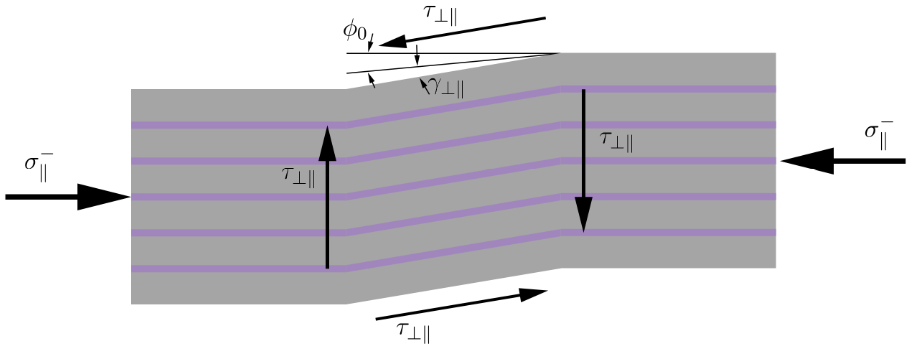
\includegraphics[width=1.0\textwidth]{Bilder/Schubknicken.png}
	\caption{Schubknicken}
	\label{fig:Schubknicken}
\end{figure} 
Schon ohne Lastangriff liegt also eine Orientierungsabweichung mit dem Winkel $\phi_0$ vor. Da trotzdem an jeder Stelle das Momentengleichgewicht herrschen muss, aber es an diesem Ort nicht mehr nur durch die Druckspannungen erfüllt ist, entstehen Schubspannungen $\tau_{\perp\parallel}$. Aus dem Momentengleichgewicht in Abbildung \ref{fig:Schubknicken} lässt sich der Zusammenhang
\begin{equation}\label{SchubknickSigma}
	\sigma_{\parallel}^-=\frac{\tau_{\perp\parallel}}{\phi_0 + \gamma_{\perp\parallel}}
\end{equation}
erkennen. Mit steigender Druckspannung steigt auch der Schiebewinkel $\gamma_{\perp\parallel}$. Bei dieser Betrachtung wurde aber noch die Biegesteifigkeit der Fasern außer Acht gelassen, die dem Schubknicken entgegenwirken. Auch die benachbarten Fasern stützen die knickenden Schichten und tragen somit zu einer erhöhten Stabilität bei. Des Weiteren ist zu beachten, dass die Schubspannung $\tau_{\perp\parallel}$ stark nichtlinear von dem Schubwinkel $\gamma_{\perp\parallel}$ abhängt. 
Die Längs-Druckfestigkeit $R_\parallel^-$ lässt sich aus der Extremwertbetrachtung von Gleichung \ref{SchubknickSigma} als der Maximalwert von $\sigma_{\parallel}^-$ zu
\begin{equation}
	R_\parallel^- = \frac{\mathrm{d}\tau_{\perp\parallel}}{\mathrm{d}\gamma_{\perp\parallel}} = G_{\perp\parallel,\mathrm{T}}(\gamma_{\perp\parallel})
\end{equation}
bestimmen. $G_{\perp\parallel,\mathrm{T}}(\gamma_{\perp\parallel})$ ist der Tangenten-Schubmodul beim Schubknicken. Wird dieser Wert überschritten, wächst der Schiebewinkel unkontrolliert an und es kommt zum lokalen Knicken, was nicht selten zum Gesamtversagen führen kann.

\noindent Häufig kommt es aber gar nicht zur Überschreitung dieser Festigkeit. Lokale Spannungsmaxima können schon vorher zum Versagen durch Zfb führen, bevor es zum Schubknicken kommt. In dem zu konstruierenden Flügel soll sich ein Holm befinden, in dessen Gurten es durch ihre relativ hohe Dicke jedoch trotzdem vorkommen kann. Somit ist dieser Fall für diese Projektarbeit nicht vernachlässigbar.

\noindent Sowohl die Längs-Druckfestigkeit $R_\parallel^-$ als auch die Längs-Zugfestigkeit $R_\parallel^+$ sind als Materialkennwerte der UD-Schicht im Rahmen der Aufgabenstellung gegeben und ergänzen die Pucksche Zigarre, indem der Bruchkörper durch diese beiden Festigkeiten in die $\sigma_1$-Richtung beschränkt wird.
\subsection{Bauweise (O.S.)}
In der Aufgabenstellung wird gefordert, dass der Flügel in der Holm-Bauweise konstruiert wird. Ein Holm besteht aus zwei parallelen Gurten, die durch einen oder mehrere Stege miteinander verbunden werden. Dabei sind verschiedene Varianten möglich. Abbildung ~\ref{fig: Holmarten} veranschaulicht Konstruktionsmöglichkeiten. Neben der Festigkeit ist die Steifigkeit die einzige strukturmechanische Anforderung. Somit lässt sich das Problem als Biegebalken betrachten, der bei der vorgegebenen Prüflast $ F_{pruef}=100\mathrm{N} $ am freien Ende die vorgegebene Durchbiegung $ w(100\mathrm{N})=22\mathrm{mm} $ einhält. Das entstehende Biegemoment wird hauptsächlich von den Gurten getragen, weswegen man sich bei der Wahl des Steges auf andere Kriterien konzentrieren kann. Da kein maximaler Drillwinkel vorgegeben ist und die Torsionssteifigkeit fast ausschließlich von der Haut bewirkt wird, führen mehrere Stege, wie man sie bei einem geschlossenen Profil hat, nur zu unerwünschter Gewichtszunahme. Nach diesen Überlegungen wurde der I-Holm ausgewählt, da dieser bei einfacher Fertigung die gewünschten Eigenschaften mit sich bringt.
\begin{figure}[h]
	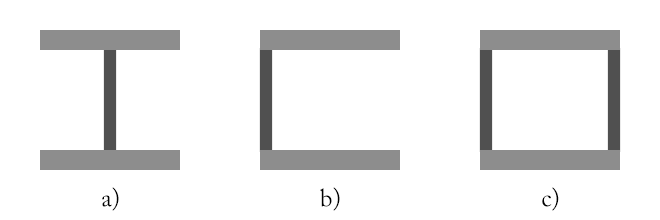
\includegraphics[width=1.0\textwidth]{Bilder/Holmarten.png}
	\caption{a) I-Holm   b) C-Holm    c) Kastenholm}
	\label{fig: Holmarten}
\end{figure}\\ 
\noindent
Das aerodynamische Profil des Flügels wird durch die Schale erreicht. Hierbei wird eine dünne Haut nur an kritischen Stellen mit der Sandwichbauweise oder Rippen verstärkt, um Beulen zu verhindern. Die Schale trägt dabei so gut wie gar nicht die Last des Flügels, jedoch ist sie für die Torsionssteifigkeit entscheidend.
